\documentclass[a4paper,12pt]{article}
\usepackage [utf8x]{inputenc}
\usepackage[czech]{babel}
\usepackage{graphicx}
\usepackage{amsmath}
\usepackage{siunitx}
\usepackage{xspace}
\usepackage{url}
\usepackage{indentfirst}
\usepackage[margin=22mm]{geometry}
\usepackage{esvect}
\usepackage{ragged2e}
\usepackage{tikz,pgf}
\usepackage{bm}
\usepackage{perpage}
\usepackage{capt-of}

\graphicspath{
	{img/}
	{plots/}
}

\MakeSorted{figure}
\newtoks\jmenopraktika \newtoks\jmeno \newtoks\datum
\newtoks\obor \newtoks\skupina \newtoks\rocnik \newtoks\semestr
\newtoks\cisloulohy \newtoks\jmenoulohy
\newtoks\tlak \newtoks\teplota \newtoks\vlhkost
\jmenopraktika={Měření prvního Townsendova koeficientu}  % nahradte jmenem vaseho predmetu
\jmeno={Radek Horňák, Lukáš Vrána}            
\datum={1. 3. 2022}        % nahradte datem mereni ulohy                           
\rocnik={2.}                  
\semestr={IV.}                 
\cisloulohy={6}    % cislo ulohy           

\begin{document}
	\begin{center}
		{\Large Přírodovědecká fakulta Masarykovy univerzity} \\
		\bigskip
		{\Large \bfseries PRAKTIKUM Z FYZIKY PLAZMATU} \\
		\bigskip
		{\Large \the\jmenopraktika}
	\end{center}
	\bigskip
	\noindent
	\setlength{\arrayrulewidth}{1pt}
	\begin{tabular*}{\textwidth}{@{\extracolsep{\fill}} l l}
		\large {\bfseries Zpracovali:}  \the\jmeno  \hspace{20mm} \large  
		{\bfseries Naměřeno:} \the\datum\\[2.5mm]
		\hline
	\end{tabular*}

\section{Teorie}

Teorie lavin popsaná Townsendem vysvětluje základní ionizační mechanismus elektrického výboje. Mějme dvě paralelní kovové desky a mezi nimi homogenní elektrické pole $E$. Elektrony jsou v poli urychlovány a sráží se s neutrálními částicemi, přičemž může docházet k nepružným srážkám vedoucím k excitaci nebo ionizaci neutrálů. Pokud počet elektronů v místě $x$ označíme $n$, pak podél dráhy d$x$ vznikne ionizačními srážkami d$n$ nových elektronů a platí

\begin{equation}
	dn = n \alpha dx
	\label{1}
\end{equation}

kde $\alpha$ je označení pro první Townsendův, někdy nazývaný i ionizační koeficient. Ten vyjadřuje počet ionizačních srážek jednoho elektronu na jednotkové délce. Integrací a následnou úpravou dostáváme vztah

\begin{equation}
	n = n_0 e^{\alpha x}
	\label{2}
\end{equation}

kde $n_0$ je počet elektronů v počátečním bodě $x$ = 0. Ionizační koeficient závisí na intenzitě elektrického pole $E$ a na tlaku plynu v aparatuře $p$. Je li $E/p$ dáno, můžeme psát $\alpha$

\begin{equation}
	\alpha = p f \frac{E}{p}
	\label{3}
\end{equation}

tedy ionizační koeficient je úměrný počtu srážek na jednotku délky. Experimentální výsledky ukazují, že konkrétní závislost $\alpha$ na $E/p$ je ve tvaru

\begin{equation}
	\frac{\alpha}{p} = A e^{-\frac{Bp}{E}} 
	\label{4}
\end{equation}

kde $A$ a $B$ jsou konstanty, pro které platí

\begin{equation}
	U_i = B/A
	\label{5}
\end{equation}

kde $U_i$ je ionizační potenciál plynu v aparatuře. Hodnotu konstant A a B lze určit experimentálně.

\section{Měření a výsledky}

Aparatura použitá v tomto praktiku schematicky znázorněná na obr. \ref{aparatura}. Její hlavní komponenty jsou zdroj napětí, rotační olejová vývěva, výbojka, jehlový ventil, Piraniho manometr, ampérmetr a voltmetr. Je založená na principu fotoelektrického jevu, pomocí rtuťové výbojky osvětlujeme hliníkovou rovinnou katodu UV zářením a produkujeme tak fotoelektrony. Ty jsou urychlovány homogenním elektrickým polem na mřížkovou anodu. Katodu můžeme posouvat a tím měnit dráhu, po níž dochází k ionizaci neutrálů. Do výbojky, kterou čerpáme vakuovou vývěvou, je vpuštěný argon. Tlak se nastavuje jehlovým ventilem a měří Piraniho manometrem. Jedná se o nepřímý manometr, pro argon je tedy tlak potřeba vynásobit faktorem 1,59.

Při měření musíme dbát na to, aby ve výbojce nevznikl samostatný výboj, tedy měříme pro hodnoty intenzity elektrického pole 80-120~V/cm. To v praxi udržujeme nastavením napětí na zdroji a přizpůsobením vzájemné vzdálenost katody a UV výbojky. Výstupem z měření je poloha katody $x$, hodnota napětí $U$ a proud $i$ pro několik hodnot konstantní intenzity elektrického pole. Pro každou změnu intenzity pole naladíme irisovou clonu UV výbojky tak, abychom měli maximální proud okolo 1800 pA z důvodu rozsahu na přístroji do 1999 pA. Proud je tedy řádově pA až nA, pro zlepšení přesnosti měření z ampérmetru odečítáme vždy 3 hodnoty a dále budeme pracovat s průměrem z nich.

V rovnici (\ref{2}) lze nahradit počet elektronů proudem. Z naměřených dat můžeme sestavit graf závislosti $i = i_0 f(x)$, viz obr. \ref{ifx} a ln$i$ = ln$i_0$ + $\alpha x$, viz obr. 



\begin{figure}[h]
	\centering
	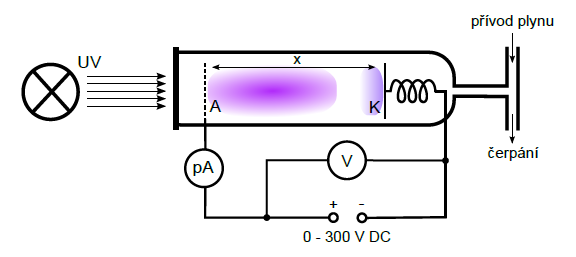
\includegraphics[width=130mm]{aparatura.png}
	\caption{Schéma použité aparatury}
	\label{aparatura}
\end{figure}

\begin{figure}[h]
	\centering
	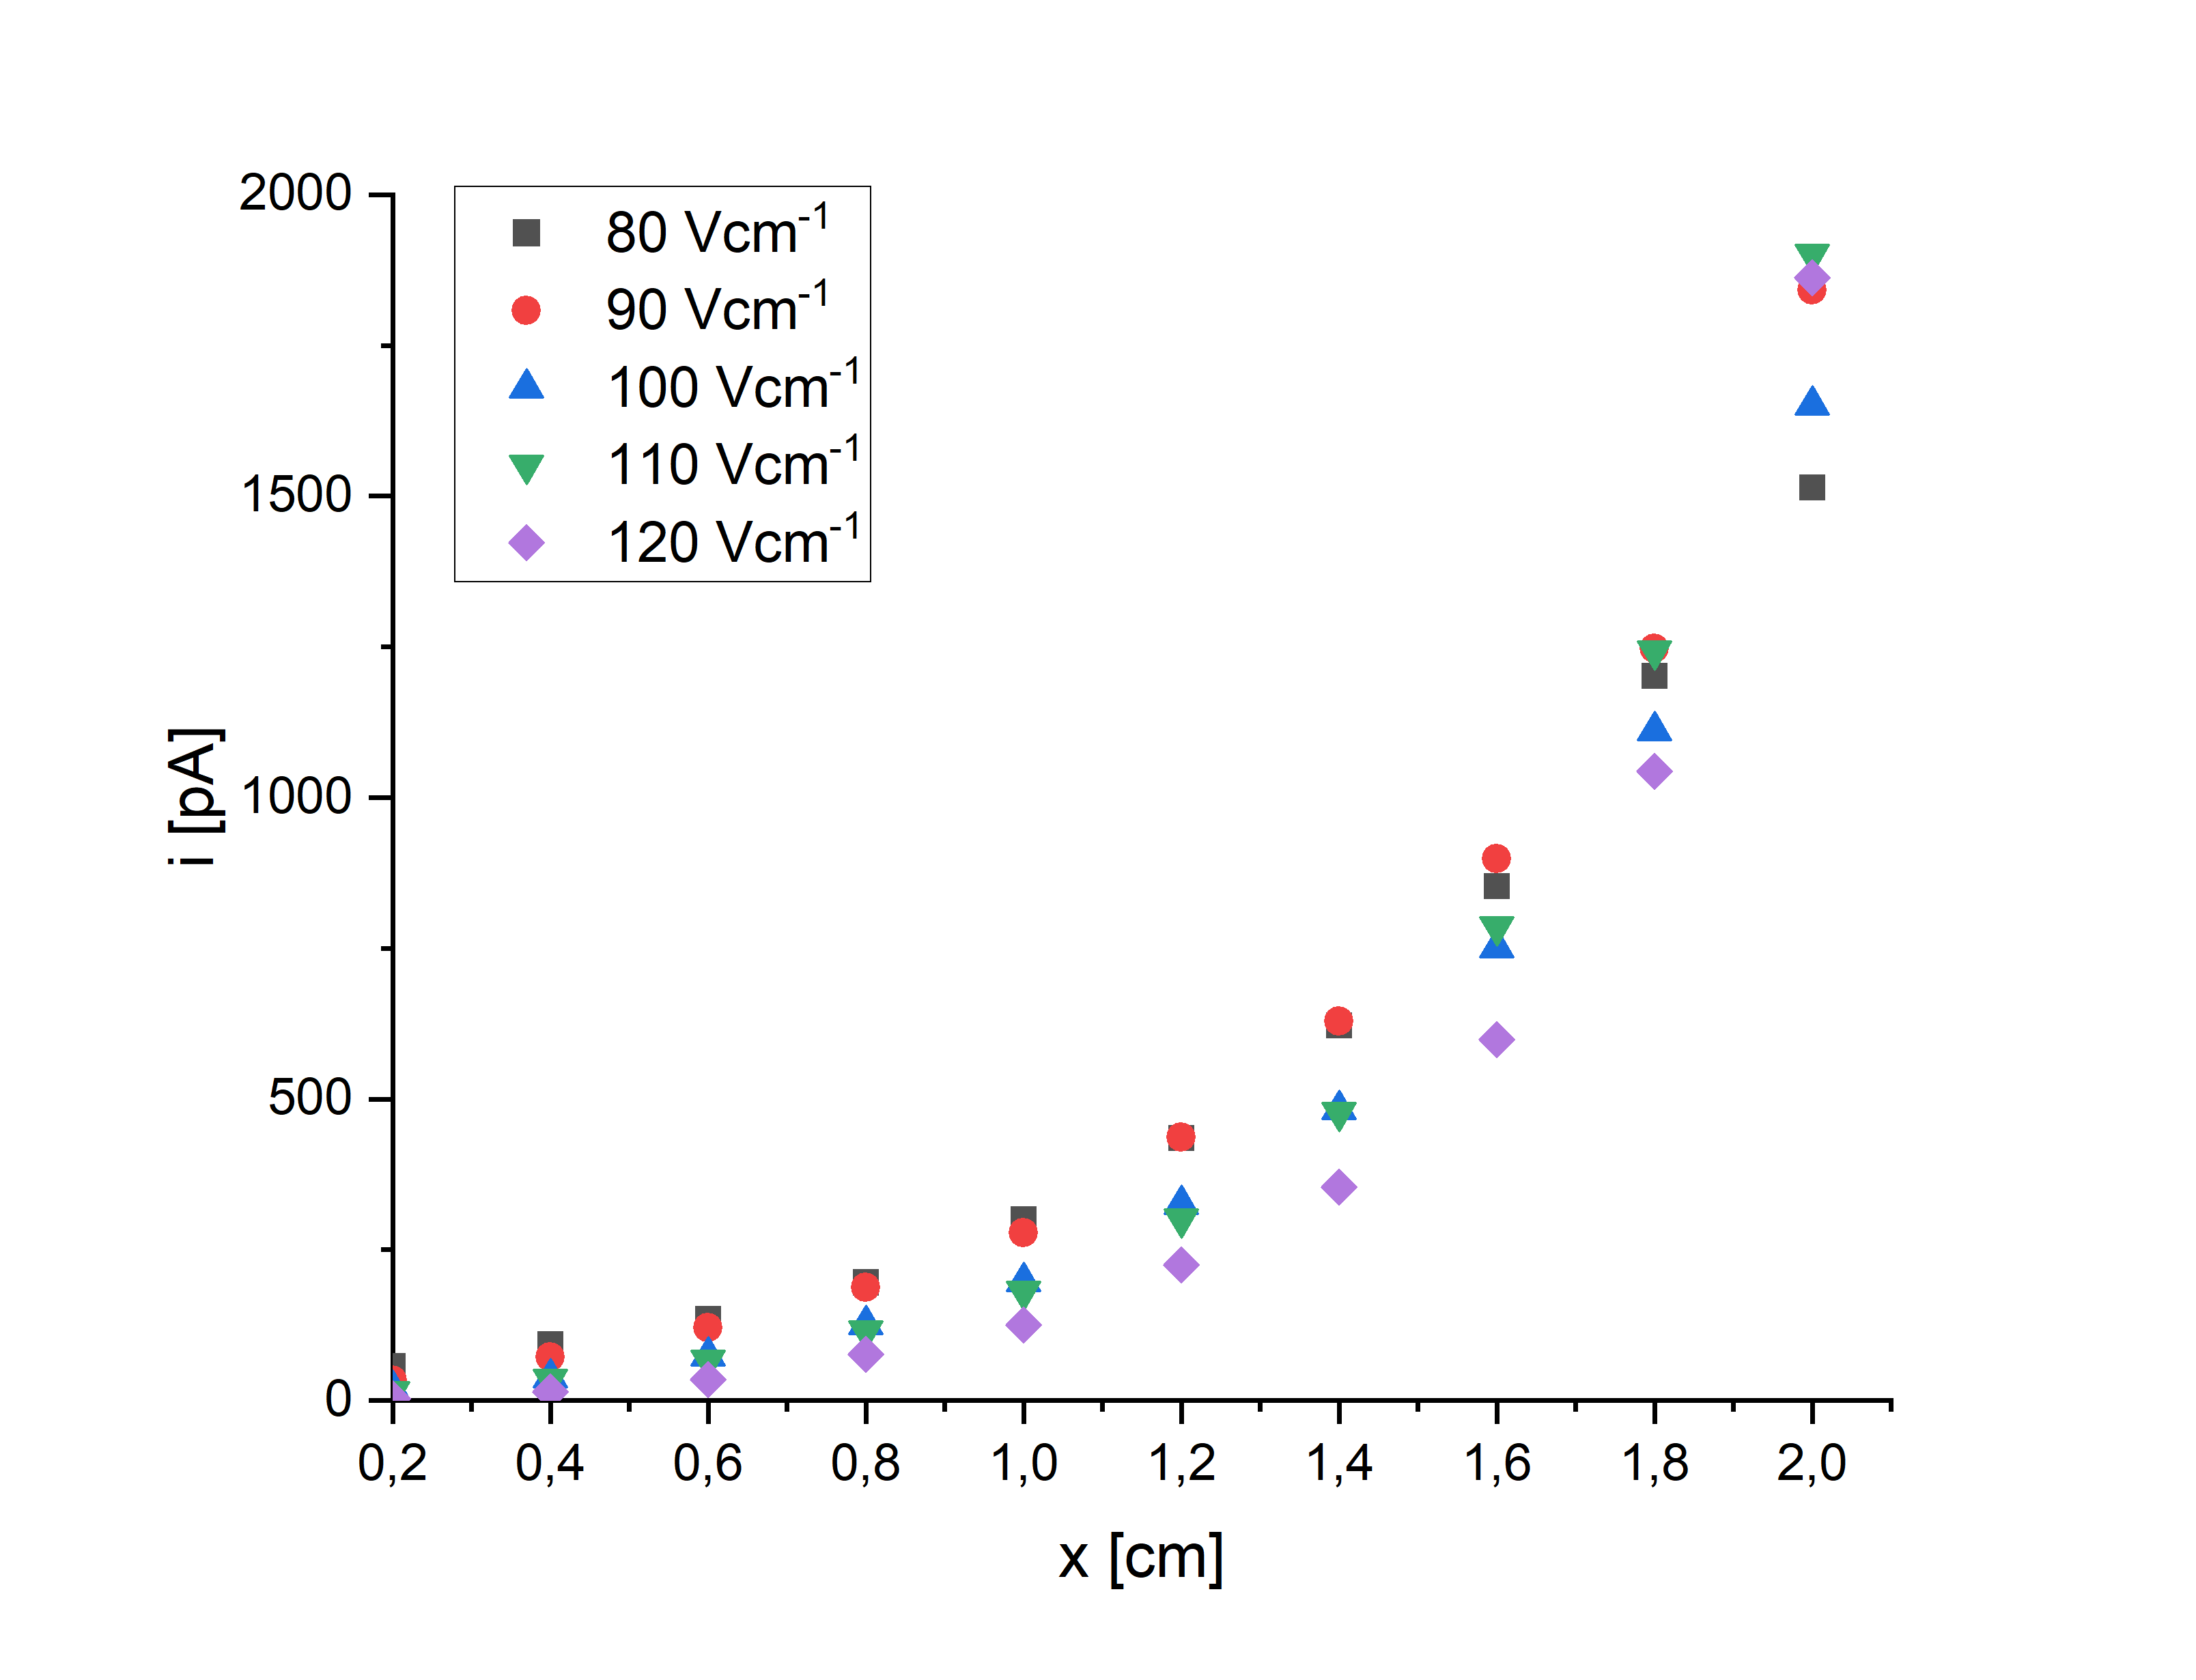
\includegraphics[width=130mm]{i=f(x).png}
	\caption{Schéma použité aparatury}
	\label{ifx}
\end{figure}


\section{Závěr}


\end{document}
